\documentclass{beamer}
% \useoutertheme[height=0pt,width=60pt,right, font=1]{sidebar}
% \usetheme[framenumber,technologie]{AP}

\usepackage[dutch]{babel}

\title[]{Embedded Systems 4}
\subtitle{}
\author{}
\institute{Jeroen Doggen \\ jeroen.doggen@artesis.be}
\date{Versie: \today}

\begin{document}

% Titlepage 
\maketitle

% Outline Page
% \section*{Overzicht}
% \begin{frame}
% \frametitle{Overzicht}
% \tableofcontents[pausesections]
% \end{frame}


%=============================================================================================================================%
\section{Inleiding}
%=============================================================================================================================%

\begin{frame} 
\frametitle{Inleiding}
Topic van dit vak:
\begin{itemize}[<+->]
 \item Embedded software development
 \item Hardware: Microsemi SmartFusion
 \item Tools
    \begin{itemize}
    \item Libero SoC: Customizable System on a Chip (cSoC) design (and simulation)
    \item SoftConsole: firmware design and debugging
    \item Putty: terminal emulator: debugging and communication
    \end{itemize}
\end{itemize}
\end{frame}

%=============================================================================================================================%

\begin{frame} 
\frametitle{SmartFusion Evaluation Board}

% \begin{itemize}
%  \item test
% \end{itemize}
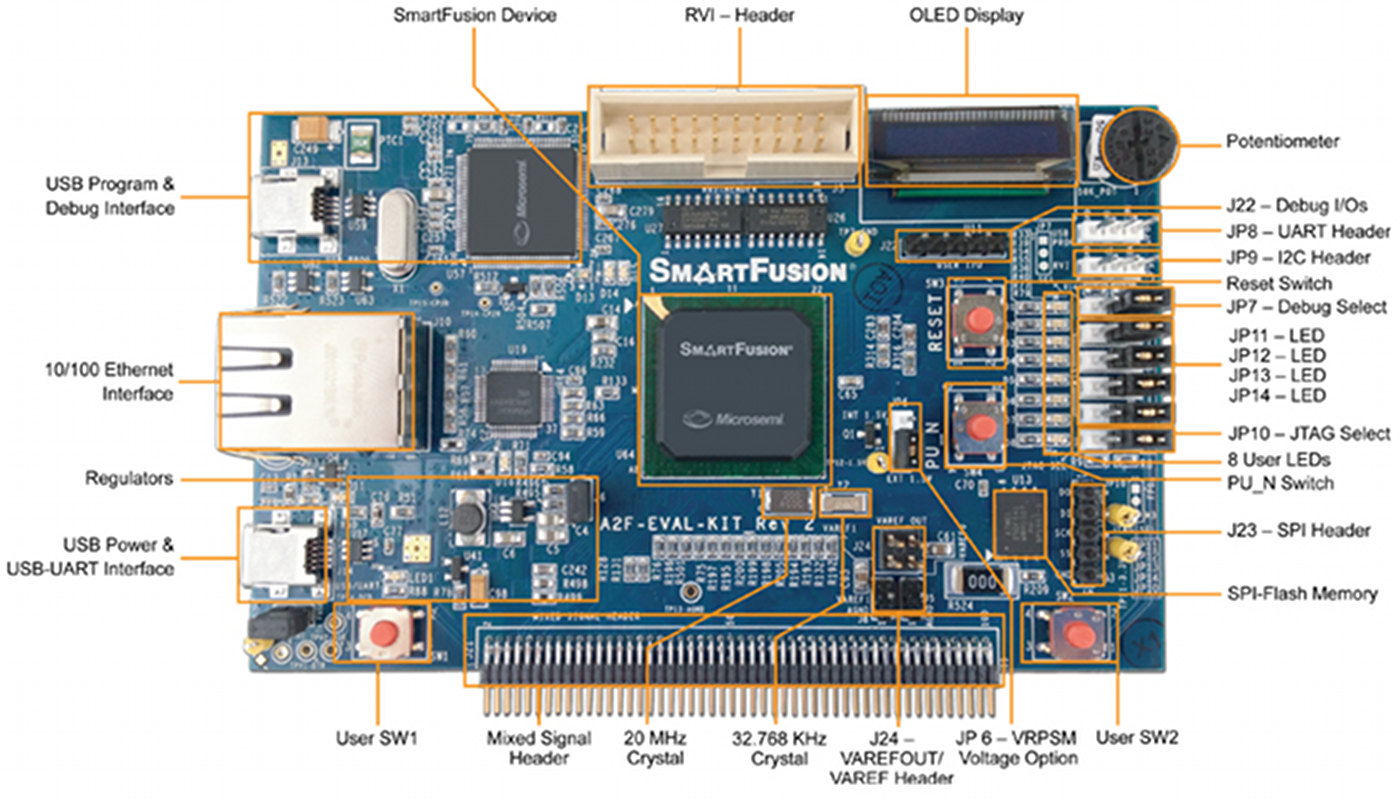
\includegraphics[width=1\textwidth]{./images/SmartFusion.jpeg}

Intro film: %\url{http://www.actel.com/FPGA/SmartFusion/video/intro_hires.html}
\url{http://www.youtube.com/watch?v=KY9eKF0llms} %(dezelfde film)
\end{frame}

%=============================================================================================================================%

\begin{frame} 
\frametitle{Embedded design flow}

\begin{itemize}[<+->]
 \item Setup a SoftConsole workspace
 \item Configure SmartFusion device
 \item Generate a sample project
 \item Program the configuration to the device
 \item Run (and debug) the program
\end{itemize}
\end{frame}

%=============================================================================================================================%

\begin{frame} 
\frametitle{Using UART with SmartFusion cSoC}
Mogelijke problemen
\begin{itemize}[<+->]
 \item Firmware nog downloaden
 \item Koppeling tussen SoftConsole en Libero niet correct
 \item Tekst in afbeeldingen en in lopende tekst is niet steeds consequent (gebruik bij voorkeur de tekst onder/boven de afbeeldingen)
 \item Broncode indenting aanpassen: code selecteren en daarna ``ctrl-i''
 \item Gebruik ``putty'' om te connecteren via de seri\"ele poort. (selecteer de juist instelling: dezelfde als gedefinieerd in de ``MSS\_UART\_init'' functie)
 \item Bij herstarten SoftConsole zijn er geen external tools beschikbaar $\rightarrow$ open eerst een workspace
 \item Bij herstarten SoftConsole is er geen debug configuration beschikbaar  $\rightarrow$ open een correct project
\end{itemize}
\end{frame}

%=============================================================================================================================%

\begin{frame} 
\frametitle{Opdracht voor les 1 \& les 2}

\begin{itemize}[<+->]
 \item Installeer Libero SoC (de standaard installatie bevat meteen ook SoftConsole)
 \item Voer de `SmartFusion SoC Quick Start Guide'' uit.
    \begin{itemize}
	\item Leer de hardware componenten configureren. (in/uit schakelen, instellen)
	\item Leren werken met de ontwikkelomgevingen.
    \end{itemize}
\end{itemize}
\end{frame}

%=============================================================================================================================%
\end{document}
%=============================================================================================================================%